\documentclass[fleqn,10pt]{olplainarticle}
% Use option lineno for line numbers 

\title{Optimizing ONNX Model Inference in a Pure C Environment for Supercomputing Applications}

\author[1]{Pedro Antunes}
\affil[1]{pedroa@kth.se}

\keywords{ONNX, MNIST, Supercomputer, OpenMP, OpenMPI}

\begin{abstract}
The field of Machine Learning (ML) continues to grow at a rapid pace, necessitating open formats like Open Neural Network Exchange (ONNX) to facilitate the sharing and utilization of ML models across diverse applications, including ML model inferencing applications. However, these applications often fail to adequately leverage the capabilities of hardware platforms where inference takes place, such as high-performance computing systems.

This work proposes an optimization approach leveraging OpenMP and OpenMPI for C-based applications targeting the Dardel supercomputer. These applications benefit from being dependency-free, offering flexibility in deployment on various hardware platforms. Notably, our implementation of an ONNX2C-based application outperformed ONNX Runtime in executing the MNIST-12 model inference, achieving an execution time of 65.28 milliseconds for ten thousand image inferences.
\end{abstract}

\begin{document}

\flushbottom
\maketitle
\thispagestyle{empty}

\section{Introduction}
The rapid expansion of machine learning and its applications creates new demands for sharing diverse models between researchers while maintaining flexibility in implementation across various hardware platforms. To address this need, open formats such as the Open Neural Network Exchange (ONNX) are essential for leveraging flexibility \cite{baiONNXOpenNeural2019}.

Despite the existence of open formats like ONNX, hardware and software choices significantly influence model performance. These choices are not always tailored to each other. In less common hardware platforms like embedded systems and supercomputers, developers would benefit from greater control over applications to leverage these systems' capabilities.

This work leverages software written in low-level languages, specifically C. This software is a set of open-source tools that enable the inference of ONNX models. These tools include cONNXr \cite{revueltaCONNXr2024}, ONNX2C \cite{kraiskilONNX2C2024}, and Libonnx \cite{xbootLibonnxLightweightPortable2024}, which are then compared with the well-established ONNX Runtime \cite{developersONNXRuntime2021}. Furthermore, this work analyzes these tools, focusing on optimizing them to execute ONNX models on the Dardel supercomputer without additional dependencies. The Dardel supercomputer comprises a CPU and GPU partition, each of which can be utilized for different computational requirements.

The CPU partition is suitable for many computational applications, while the GPU partition is more suited for straightforward yet computationally demanding tasks. This work takes advantage of the CPU partition and explores the parallelism that can be obtained from the 1278 nodes in Dardel, each equipped with two AMD EPYC Zen2 64-core processors. This parallelism is leveraged by utilizing OpenMPI \cite{gabrielOpenMPIGoals2004} and OpenMP (Open Multi-Processing) \cite{dagumOpenMPIndustryStandard1998}.

At the conclusion of this study, we aim to have a comprehensive understanding of which software tools are best suited for inferencing ONNX models in constrained environments, deviating from typical systems. To achieve this objective, we set out to accomplish the following goals through this work:
\begin{itemize}
    \item A thorough comprehension of the cONNXr, ONNX2C, and Libonnx software;
    \item An understanding of how to effectively leverage OpenMP and OpenMPI in a pure C environment to utilize the resources available at Dardel;
    \item A performance comparison between the original ONNX runtime and the optimized pure C software tools developed in this work;
    \item Identify a software solution that can be easily adapted to exploit the system resources in uncommon hardware platforms fully. 
\end{itemize}

The rest of this document is organized as follows: Section 2 describes the methodologies employed for evaluating the performance of each application, detailing the optimizations made to the serial code; Section 3 presents the results obtained from running MNIST-12 model inference on the different applications; and finally, Section 4 discusses the obtained results and concludes this work.

\section{Background}
This Section provides an overview of the software tools employed in this research, highlighting their key features and functionalities.

Firstly, ONNX is an open format for representing and sharing machine learning models between different frameworks and environments. This open format allows developers to export models from one framework like TensorFlow \cite{martinabadiTensorFlowLargescaleMachine2015} or PyTorch \cite{paszkePyTorchImperativeStyle2019} and import them into another without having to rewrite or recompile the model. Leveraging this tool facilitates machine learning researchers deploying their models in multiple platforms without knowing in detail how the framework that runs them works.

Subsequently, the ONNX Runtime software is an open-source inference engine developed by Microsoft. Various programming languages leverage this framework, which allows for the efficient execution of machine-learning models. By leveraging ONNX Runtime, users can seamlessly load and execute pre-trained models and input tensors and perform inferencing operations without requiring detailed knowledge of the underlying implementation.

The CONNXr software is an ONNX runtime application implemented in pure C. Diverging from the ONNX Runtime, which serves as a framework for function calls, CONNXr operates as a standalone executable that is compiled and then invoked directly, passing the ONNX model and input data as arguments. Besides these arguments, the user can optionally provide the `--dump-file` argument so that the program generates an output file with the results after executing each layer of the NN model. Like ONNX Runtime, CONNXr requires an operating system to execute; however, it does not rely on any additional dependencies

The ONNX2C software is a converter tool that transforms an ONNX model into equivalent C functions and produces a "model.c" file. In contrast to the other software, the ONNX2C source files are not required after generating this C file. Nevertheless, supplementary code must be developed to allow user interaction, including input loading, starting the model inference, and reading the output from the ONNX model. Among the generated functions is "entry(...)", which represents the primary entry point for executing inference within this converted model. This function receives two parameters: the input and output tensor of the model. Afterward, it orchestrates the invocation of all corresponding functions associated with the various layers of the converted model.

The Libonnx software is a runtime library that enables the use of ONNX models in various applications. Compiling its source files allows a library to be generated and subsequently integrated into a custom application. To effectively harness the capabilities of this software, a program must be developed that incorporates both the compiled library and the ONNX header file. This program should load the ONNX model and input tensor, followed by the execution of the function initiating image inferencing. Subsequently, the functions corresponding to the model layers present in the compiled library are invoked as necessary, enabling seamless integration with the custom application.

Moreover, the performance of these software tools is analyzed using Valgrind \cite{nethercoteValgrindProgramSupervision2003} and KCachGrind \cite{weidendorferSequentialPerformanceAnalysis2008}. Valgrind is an open-source profiling tool that allows developers to gain a better understanding of their applications, such as memory leaks and performance issues. This tool can be executed with the `--callgrind` argument. Passing this argument creates an output file that details how many times a certain function is called and how many instructions each function runs when it is called. KCachGrind can be used to visualize this data and determine the most resource-consuming parts of an application.

Notably, the MNIST-12 model and the MNIST dataset \cite{lecunMNISTHandwrittenDigit2010} are used to test these tools. This model and dataset can be considered the hello world application when developing NN applications, and it contains handwritten digits (0-9). This dataset consists of 70,000 images of size 28x28 pixels, divided into a training set (60,000 images) and a test set (10,000 images). Each image is labeled with the corresponding digit class (0-9), allowing us to test our software on this well-defined problem.

Finally, the software studied in this work can be optimized using OpenMPI and OpenMP, which leverage the CPU resources available on Dardel. These tools allow the parallelization of the code by leveraging the available cores in the system. Specifically, OpenMPI is more suitable for parallelizing software at a higher level within an application's top layers. As an open-source implementation of the Message Passing Interface (MPI) standard for parallel computing, it enables users to write programs that can execute in parallel across multiple processes or nodes on high-performance computing systems. In contrast, OpenMP is better suited for parallelizing the inner functionalities of applications. This API supports multi-platform shared memory parallel programming in C, C++, and Fortran, utilizing compiler directives (pragmas), runtime library routines, and environment variables to control the execution of parallel code.

\section{Methods}
This section outlines the methodology and key decisions made in this work. Initially, a comprehensive review of existing applications for running inference on ONNX models was conducted, focusing on selecting an application worthy of further investigation. Notable candidates from this review included well-known frameworks such as ONNX Runtime, ONNX-MLIR \cite{onnxOnnxmlir2024}, OpenVino \cite{openvinotoolkitOpenvino2024}, and TensorFlow, as well as lesser-known alternatives like cONNXr, ONNX2C, and Libonnx. This latter group, written in pure C without multi-threading or GPU optimization, presented an opportunity to explore the benefits of optimizing their serial code using OpenMP and OpenMPI. Given that more well-known applications already incorporate methods for leveraging available resources, a comparative analysis was performed between these applications and ONNX Runtime.

Subsequently, the choice of AI model and dataset was made. In this context, the objective is to evaluate performance optimization techniques on pure C applications, thereby enabling readers to compare results with those from other studies easily. A concrete and well-tested dataset and model were selected for this purpose.

Furthermore, a thorough analysis of the chosen application codes was conducted to identify key optimization areas. Custom wrapper programs were developed to validate the correct functionality of these applications and benchmark their performance. Moreover, this analysis also involved utilizing Valgrind and KCachegrind, two widely used open-source debugging and performance analysis tools. 

\subsection{AI model and Dataset}
The selected model for this study was the pre-trained MNIST-12 model, available at the ONNX models repository on GitHub (https://github.com/onnx/models/tree/main/validated/vision/classification/mnist). This model utilizes ONNX version 1.9 and is readily available for use. This model architecture can be effectively visualized using the Netron application \cite{lutzroederNetron2024}, enabling a clear representation of its constituent layers, as seen in Figure \ref{fig:mnist_12_model}.

\begin{figure}[!ht]
    \centering
    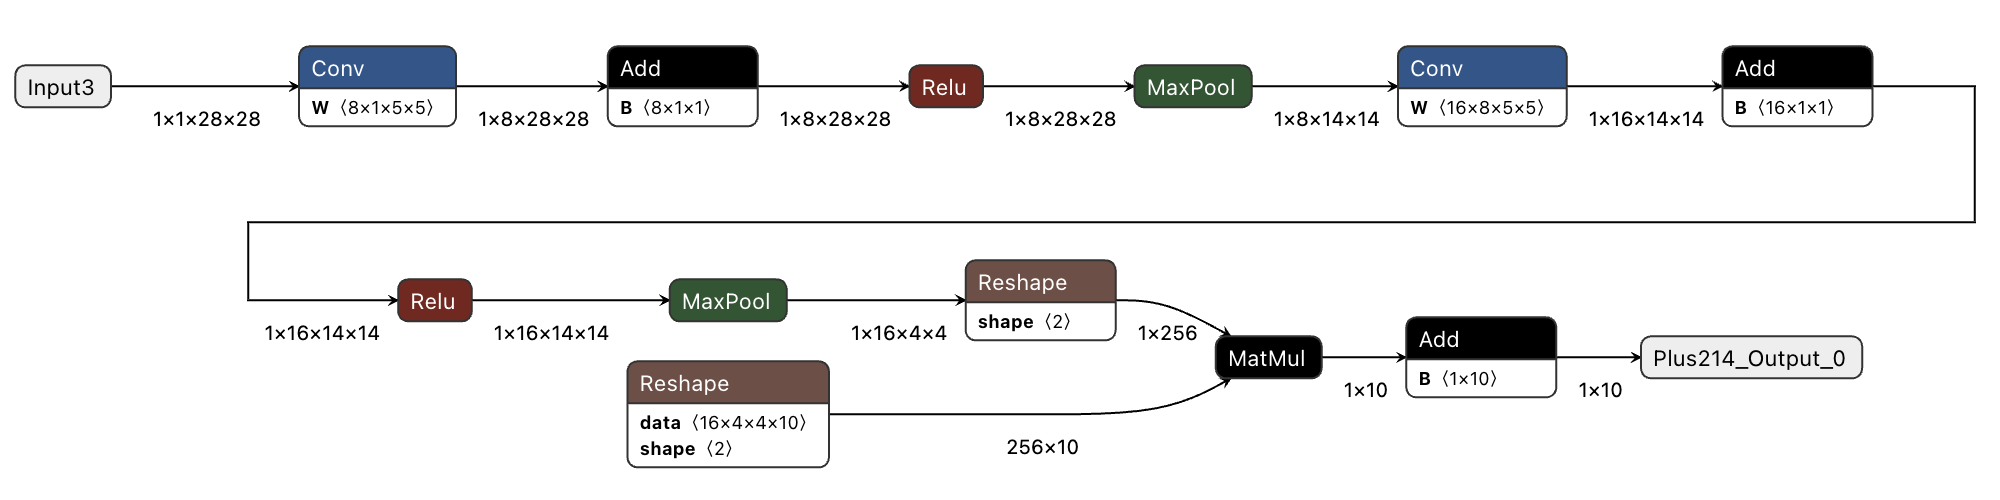
\includegraphics[width=\textwidth]{Images/mnist_12_model.png}
    \caption{Visualization of the MNIST-12 Model Layers Using Netron.}
    \label{fig:mnist_12_model}
\end{figure}

The accompanying dataset is the MNIST dataset, comprising a handwritten digit image collection. Only the testing data from this dataset, consisting of 10,000 images, was utilized for this study. These images can be obtained using PyTorch from https://ossci-datasets.s3.amazonaws.com/mnist/t10k-images-idx3-ubyte.gz and their corresponding labels from https://ossci-datasets.s3.amazonaws.com/mnist/t10k-labels-idx1-ubyte.gz. Alternatively, one test input and the corresponding expected output of this dataset are also provided alongside the model from the onnx repository.

The input data for the model consists of a single 28x28 pixel image, while the output data is an array of 10 floating-point values. Each value in this array represents the probability that the input image corresponds to a specific digit, with the index of each value matching the corresponding digit. Therefore, by analyzing the output data, it is possible to determine which digit the model predicts the input image to represent.

\subsection{Inference}
Image inferencing of the MNIST dataset was performed and benchmarked in four distinct applications. Initially, an approach utilizing ONNXRuntime was implemented, which can leverage CPU multi-threading and GPU acceleration to achieve improved performance.  This approach served as the baseline for subsequent evaluations. Subsequently, the serial code of three C-based applications was thoroughly analyzed and optimized with the goal of outperforming the performance obtained by ONNXRuntime.

Our analysis revealed that incorporating parallel zones of code using OpenMP can result in a significant overhead, particularly when creating numerous threads within nested loops. This observation holds true for all examined applications, underscoring the importance of carefully selecting optimization techniques to avoid performance degradation. Furthermore, the design and structure of these applications' code significantly impact their adaptability and optimizability.

All developed code for this project is publicly available on the authors GitHub repository: 

https://github.com/PedroAntunes178/PDC\_Project\_2024.git.

\subsubsection{ONNXRuntime}
A Python virtual environment was created to create a development environment setup with ONNXRuntime and numpy version 1.24. Following this setup, we proceeded to utilize ONNX Runtime for inference tasks. A Python script was developed to load the model and the input image and execute inference. This script also measured the time required to process one image (inference time) and validated whether the output conformed to the expected result. Notably, the inference was executed using the CPU, as per the ONNXRuntime documentation, which defaults to utilizing all available cores in a system. Given Dardel's configuration featuring two AMD EPYC Zen2 2.25 GHz 64-core processors per node, with no inter-processor or node communication implemented.

The input data utilized in this experiment, which served as a test case, is a single image sourced from the ONNX repository. Our developed script records the inference time for this image, and upon executing the script multiple times with sufficient temporal gaps between runs to prevent data caching, the minimum reported inference time was selected as the benchmark for this application's performance and optimization target for the other applications.

\subsubsection{cONNXr}
Initially, the ConXr program is run as-is after being cloned from GitHub. The MNIST-12 model and input data (corresponding to one test image) are passed as arguments, along with the `--dump-file` flag for debugging purposes. This allows for analysis of the correct program behavior by comparing the output file with results obtained at each layer, specifically the last layer's output and expected output accompanying the input data.

Subsequently, application performance was analyzed using Valgrind, invoked with the `--callgrind` argument. This argument enables verification of which parts of the code consume the most CPU processing power during execution. The resulting data is visualized in Figures \ref{fig:connxr_tree} and \ref{fig:connxr_ir}, indicating that the `execute\_operator\_\_ai\_onnx\_\_conv\_\_11\_\_T\_float(...)` function accounts for 95.96\% of executed instructions, thereby identifying the most consuming function within the application.


\begin{figure}[!ht]
    \centering
    \begin{subfigure}[b]{0.4\textwidth}
        \centering
        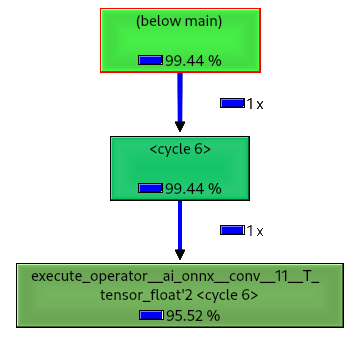
\includegraphics[width=\textwidth]{Images/connxr.png}
        \caption{Call graph visualization from KCacheGrind illustrating the flow and time consumption of functions in the MNIST-12 model inference.}
        \label{fig:connxr_tree}
    \end{subfigure}
    \hfill
    \begin{subfigure}[b]{0.45\textwidth}
        \centering
        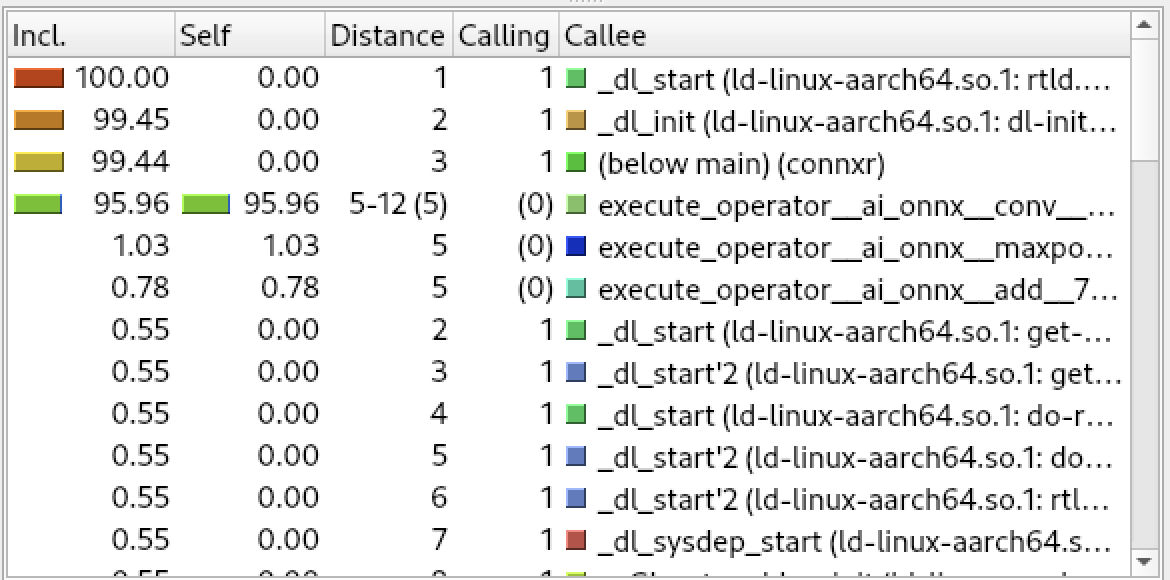
\includegraphics[width=\textwidth]{Images/connxr_ir.png}
        \caption{Annotated function call list from KCacheGrind showing the time distribution across various operations in the MNIST-12 model inference.}
        \label{fig:connxr_ir}
    \end{subfigure}
    \caption{Performance profiling of a cONNXr-based application using KCacheGrind. The function \textit{execute\_operator\_\_ai\_onnx\_\_conv\_\_11\_\_T\_float} consume the most computational resources, indicating a potential area for optimization.}
    \label{fig:connxr}
\end{figure}

After analyzing the performance data and source code, we optimized the most resource-intensive function using OpenMP. This function implements convolution layers in ONNX models, utilizing 32-bit floating-point arithmetic. Notably, this function is invoked whenever a convolution layer exists within the model. The MNIST-12 model comprises two convolution layers, resulting in this function being called twice in the code. This behavior can be verified through Valgrind data and by adding print statements at the beginning of the function.

The parallelizable portion of this function lies within its for loops, which iterate over convolution kernels and input feature maps. Using OpenMP, we employed a `\#pragma omp parallel for` directive to parallelize these loops. To optimize thread utilization, we appended the following clauses:
\begin{itemize}
    \item `collapse(4)`: This clause collapses the four nested for loops, distributing their workload evenly across available threads. To achieve this, a variable computation was relocated from an outer loop to an inner loop.
    \item `private(n, m, b, k, i, j)`: These variables are declared private to each thread, ensuring independence and eliminating data contention.
    \item `firstprivate(h\_kernel, w\_kernel)`: This clause initializes the h\_kernel and w\_kernel variables with their values before the OpenMP pragma (in thread 0), maintaining consistency across threads.
\end{itemize}

We added the OMP library at the beginning of the C file containing the convolution function to compile the program with OpenMP support. The original Makefile was also modified by appending `-fopenmp` to the compilation flags.

\subsubsection{ONNX2C}
Like the other approaches, the first step was to run this application in serial. With this application, a C file corresponding to the MNIST-12 model was generated to accomplish this step. This is followed by creating a main C file that loads a dataset comprising 10,000 images and calls the converted model to perform inference on each image individually. The inference process was initiated by calling the entry function of the converted MNIST-12 model with the input image (28x28 pixels) and the output memory location.

Following the execution of the serial code, we conducted a performance analysis using Valgrind and KCacheGrind. This process is similar to that of other applications. This analysis revealed that the code executed most of the instructions when processing the two convolution layers present in the MNIST-12 model (Figure \ref{fig:mnist_12_model}). The data from this analysis is visualized in Figures \ref{fig:onnx2c_tree} and \ref{fig:onnx2c_ir}.

\begin{figure}[!ht]
    \centering
    \begin{subfigure}[b]{0.45\textwidth}
        \centering
        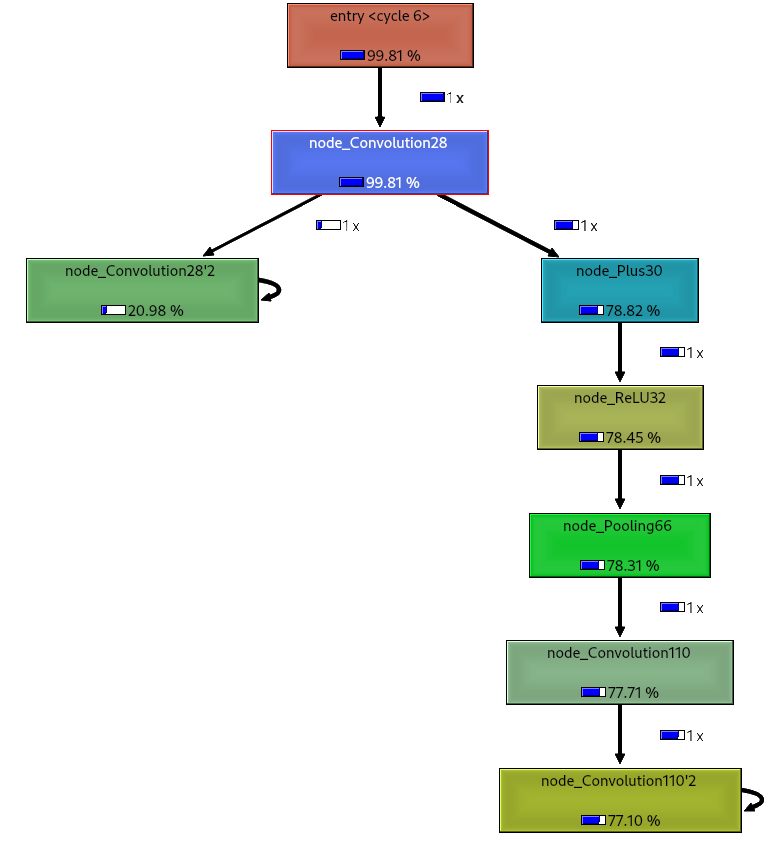
\includegraphics[width=\textwidth]{Images/onnx2c.png}
        \caption{Call graph visualization from KCacheGrind illustrating the flow and time consumption of functions in the MNIST-12 model inference.}
        \label{fig:onnx2c_tree}
    \end{subfigure}
    \hfill
    \begin{subfigure}[b]{0.45\textwidth}
        \centering
        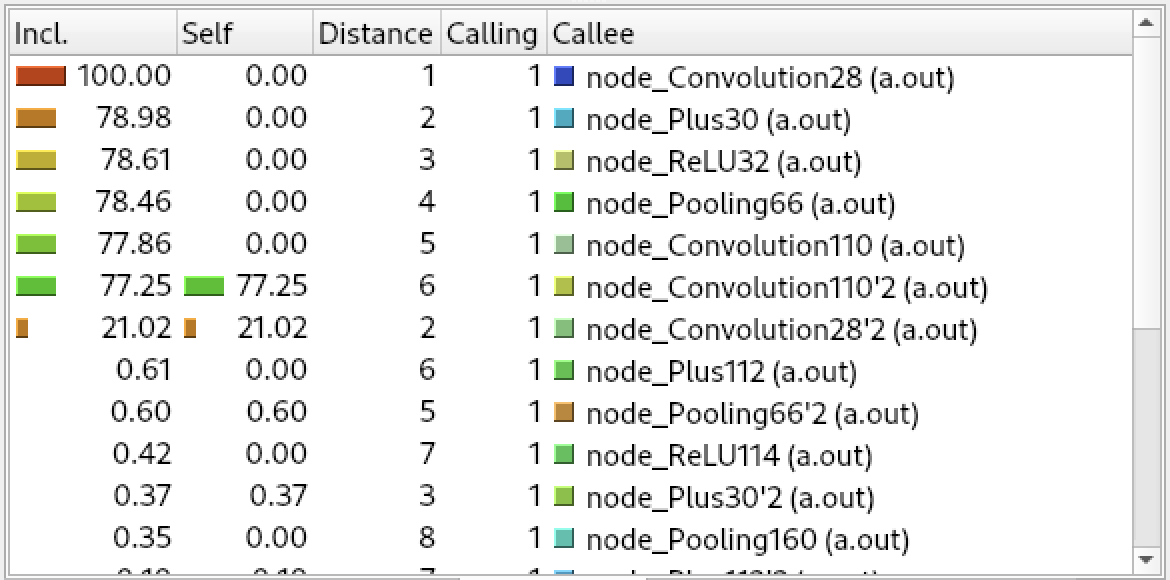
\includegraphics[width=\textwidth]{Images/onnx2c_ir.png}
        \caption{Annotated function call list from KCacheGrind showing the time distribution across various operations in the MNIST-12 model inference.}
        \label{fig:onnx2c_ir}
    \end{subfigure}
    \caption{Performance profiling of a onnx2c-based application using KCacheGrind. The functions \textit{node\_Convolution110}, and \textit{node\_Convolution28} consume the most computational resources, indicating potential areas for optimization.}
    \label{fig:onnx2c}
\end{figure}

As observed in Figure \ref{fig:onnx2c_tree}, the compiler optimized the code such that each function did not return to the entry function upon completion but instead called the next layer of the model. Furthermore, according to this performance analysis and as depicted in Figure \ref{fig:onnx2c_ir}, 77.10\% of the instructions were executed by the Convolution110 layer, which is the second convolution layer of the model. Consequently, this function was identified as the most relevant one for optimization.

To achieve optimization, we employed OpenMP to split the workload of the for loops within the corresponding C function between different threads. This optimization utilized a `\#pragma omp parallel for` directive with the clause `collapse(4)`, which distributed the workload of the four loops evenly across available threads. To enable this computation, the for loops generated by the application were slightly adapted such that some operations were explicitly computed in the inner loop.

Following the initial optimization, we further optimized the first convolution layer (Convolution28) to improve performance when running inference on a single image. This layer execution corresponds to 21.02\% of the instructions executed. This optimization was identical to the previous one.

Another optimization approach employed in this application was batch parallelization. Instead of performing inference on a single image at a time, multiple images were processed in parallel across different cores or CPUs using OpenMPI. This level of parallelism was achieved in the main function, where MPI was initialized, and the images were distributed among each rank. The distribution was performed by splitting the total number of images (n\_images) by the number of processes launched with the MPI application. As a result, each rank received $\frac{n\_images}{n\_processes}$ images, with any remaining images assigned to the last rank.

During inference, each rank counted the number of correct and incorrect classifications by comparing against the expected labels. Upon completion, the results were shared among ranks using the MPI\_Reduce function, allowing for the accumulation and aggregation of results in rank 0. Subsequently, each non-zero rank sent its measured inference time to rank 0. To prevent stalling, rank 0 awaited messages from any source, as some ranks may take longer than others to complete their tasks. This approach enabled optimal performance. When receiving these messages this rank stores the maximum inference time, curresponding to the rank that took the longest to complete inference. After gathering this information this rank (rank 0) calculats and prints the model's accuracy, confirming its correct behavior, as well as the overall inference time.

\subsubsection{Libonnx}
Similar to other approaches, the first step involved executing image inference from the MNIST dataset utilizing the MNIST-12 model. This process entailed compiling source files and generating a libonnx.a file, followed by creating a primary C file containing the main function. The latter loaded the model and input tensor, initiated model inference, and concurrently tracked inference time while verifying output conformity to expected results.

Performance analysis of this program revealed that three functions accounted for the majority of executed instructions. Notably, the most computationally intensive function was the convolutional operation, which comprised 45.73\% of total instructions, as depicted in Figures \ref{fig:libonnx_tree} and \ref{fig:libonnx_ir}. The other two most demanding functions were Add\_float32 and MaxPoll\_float32, corresponding to matrix addition nodes and polling layers within the model.

\begin{figure}[!ht]
    \centering
    \begin{subfigure}[b]{0.45\textwidth}
        \centering
        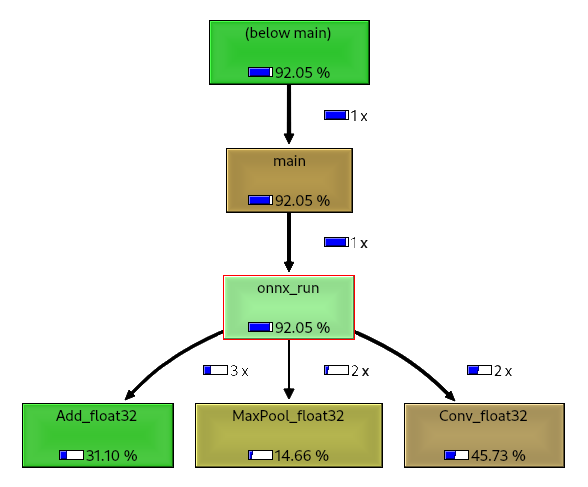
\includegraphics[width=\textwidth]{Images/libonnx.png}
        \caption{Annotated function call list from KCacheGrind showing the time distribution across various operations in the MNIST-12 model inference.}
        \label{fig:libonnx_tree}
    \end{subfigure}
    \hfill
    \begin{subfigure}[b]{0.45\textwidth}
        \centering
        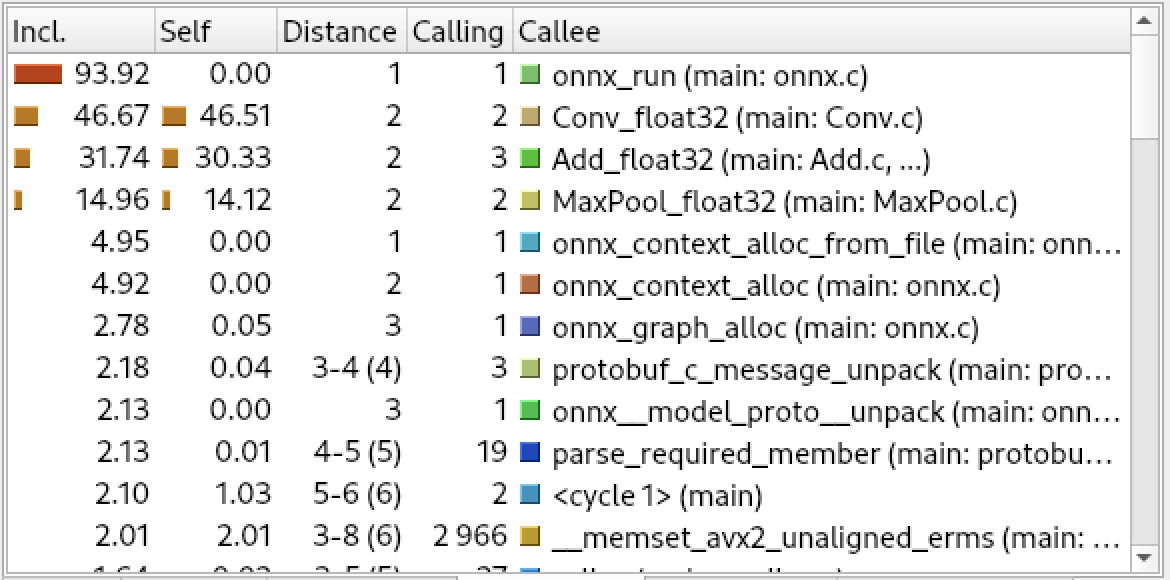
\includegraphics[width=\textwidth]{Images/libonnx_ir.png}
        \caption{Call graph visualization from KCacheGrind illustrating the flow and time consumption of functions in the MNIST-12 model inference.}
        \label{fig:libonnx_ir}
    \end{subfigure}
    \caption{Performance profiling of a Libonnx-based application using KCacheGrind. The functions \textit{Conv\_float32}, \textit{Add\_float32}, and \textit{MaxPool\_float32} consume the most computational resources, indicating potential areas for optimization.}
    \label{fig:libonnx}
\end{figure}

Subsequent experimentation with OpenMP for parallelization of this software yielded no performance enhancements. Consequently, an optimized version of the software was not developed.

\section{Experimental Results}
This section provides an overview of the outcomes achieved by executing the experiments designed in this study. These experiments consisted of running inferences on images from the MNIST dataset within the applications analyzed, with optimizations tested by varying the number of OMP threads and the number of MPI processes. This latter value is changed by changing the number of nodes and/or processes per node used.

Firstly, we present a comparison of the results obtained from running the serial implementations of the analyzed applications, as presented in Table \ref{tab:all_serial}. These results demonstrate that the ONNX Runtime application achieves the best performance, with a small gap between it and cONNXr and Libonnx. Notably, while the other applications are fully sequential, the ONNX Runtime attempts to implement thread parallelism, making this gap intriguing. 

\begin{table}[!ht]
    \centering
    \begin{tabular}{|l|c|}
    \hline
    \textbf{Application} & \textbf{Inference time (ms)} \\ \hline
    ONNXRuntime          & 0.890                        \\ \hline
    cONNXr               & 1.370                        \\ \hline
    ONNX2C               & 4.267                        \\ \hline
    Libonnx              & 1.162                        \\ \hline
    \end{tabular}
    \caption{Comparison of Inference Times for One Image from the MNIST Dataset.}
    \label{tab:all_serial}
\end{table}
%![[Pasted image 20241015092125.png]]

Upon analyzing the source code, we conclude that this disparity arises from the fact that cONNXr and Libonnx employ code optimizations that cache model and intermediary feature maps. By leveraging these caches more effectively, these applications can access memory faster and achieve better performance. Additionally, this slight performance difference observed can be attributed to the simplicity of the ONNX model used for testing. This model utilizes few memory resources, making it easier to cache, and does not implement very complex layers.

In contrast, the ONNX2C software does not consider caching and is noticeably slower than the other solutions.

Subsequently, we present and discuss the optimizations performed in the applications leveraging cONNXr and ONNX2C. These optimizations reveal that a simpler application architecture enables effortless navigability and flexibility to leverage available system resources effectively.

\subsection{cONNXr}
The optimizations performed on the cONNXr software revealed that optimal performance was achieved when the program was launched with four OMP threads, as evident in Table \ref{tab:connxr_omp}. This outcome can be attributed to the small size of the model being executed, which renders additional OMP threads unnecessary. Consequently, spawning and deleting excess threads incurs an overhead, thereby negating any potential performance benefits.

\begin{table}[!ht]
    \centering
    \begin{tabular}{|l|c|}
    \hline
    \textbf{OMP number of threads} & \textbf{Inference time (ms)} \\ \hline
    1                              & 1.37                         \\ \hline
    2                              & 1.139                        \\ \hline
    4                              & 0.977                        \\ \hline
    8                              & 1.206                        \\ \hline
    16                             & 2.14                         \\ \hline
    32                             & 3.543                        \\ \hline
    64                             & 67.195                       \\ \hline
    \end{tabular}
    \caption{Inference of One MNIST Image for cONNXr Utilizing OpenMP Parallelization.}
    \label{tab:connxr_omp}
\end{table}
%![[Pasted image 20241015205419.png]]

\subsection{ONNX2C}
The results of optimizations conducted on software utilizing ONNX2C are presented in this subsection. Performance enhancements leveraging OpenMP, OpenMPI, and their concurrent application are demonstrated. In the course of performance analysis, we executed inference on 10000 images, annotating the time required to accomplish this task. The inference time for a single image was calculated by dividing this value by 10000. This inference time is the value reported in the tables.

Our experimental results demonstrate that utilizing OpenMP to leverage all available cores within a node yields optimal performance, as illustrated in Table \ref{tab:onnx2c_omp}. We conducted two separate experiments to investigate the impact of optimizing multiple layers. Initially, only the largest convolutional layer was optimized, followed by an additional experiment where both the first and second convolutional layers were optimized.

Comparative analysis reveals that when utilizing two OpenMP threads, optimizing the second layer has a negligible effect on performance. Conversely, as the number of OMP threads is increased, the weight of the unoptimized convolutional layer becomes significantly noticeable in terms of inference time.

\begin{table}[!ht]
    \centering
    \begin{tabular}{l|cc|}
    \cline{2-3}
    \textbf{}                                            & \multicolumn{2}{c|}{\textbf{Inference time (ms)}}                                        \\ \hline
    \multicolumn{1}{|l|}{\textbf{OMP number of threads}} & \multicolumn{1}{c|}{\textbf{One layer parallelized}} & \textbf{Both layers parallelized} \\ \hline
    \multicolumn{1}{|l|}{1}                              & \multicolumn{1}{c|}{4.47634}                         & 4.89509                           \\ \hline
    \multicolumn{1}{|l|}{2}                              & \multicolumn{1}{c|}{2.78428}                         & 2.52732                           \\ \hline
    \multicolumn{1}{|l|}{4}                              & \multicolumn{1}{c|}{1.90613}                         & 1.37494                           \\ \hline
    \multicolumn{1}{|l|}{8}                              & \multicolumn{1}{c|}{1.4732}                          & 0.78213                           \\ \hline
    \multicolumn{1}{|l|}{16}                             & \multicolumn{1}{c|}{1.25739}                         & 0.49739                           \\ \hline
    \multicolumn{1}{|l|}{32}                             & \multicolumn{1}{c|}{1.15571}                         & 0.35527                           \\ \hline
    \multicolumn{1}{|l|}{64}                             & \multicolumn{1}{c|}{1.12415}                         & 0.34691                           \\ \hline
    \multicolumn{1}{|l|}{128}                            & \multicolumn{1}{c|}{1.11333}                         & 0.34596                           \\ \hline
    \end{tabular}
    \caption{Inference Time per Image for ONNX2C Utilizing OpenMP Parallelization.}
    \label{tab:onnx2c_omp}
\end{table}
%![[Pasted image 20241015205451.png]]

These experiments have demonstrated that this optimized application achieves excellent performance by utilizing OpenMP. This performance improvement is a speedup of 2.57x relative to ONNX Runtime's inference time. Furthermore, the inherent characteristics of our application enable leveraging batch parallelism, allowing for additional performance improvements through concurrent execution of multiple input batches.

These performance improvements can be achieved by leveraging parallel processing capabilities using OpenMPI. As demonstrated in Tables \ref{tab:onnx2c_mpi}, the optimal performance is achieved when utilizing as many processes as possible. This outcome is consistent with expectations, as the increased number of cores enables the efficient division of the 10,000 images among multiple processing units. Notably, further improvements in inference time are contingent upon increasing the number of nodes to accommodate additional cores, thereby facilitating simultaneous utilization and maximizing overall performance.

\begin{table}[!ht]
    \centering
    \begin{tabular}{|l|c|}
    \hline
    \textbf{MPI number of processes} & \textbf{Inference time (ms)} \\ \hline
    2                                & 2.389876                     \\ \hline
    4                                & 1.206962                     \\ \hline
    8                                & 0.602174                     \\ \hline
    16                               & 0.300168                     \\ \hline
    32                               & 0.151566                     \\ \hline
    64                               & 0.076452                     \\ \hline
    \end{tabular}
    \caption{Inference Time per Image for ONNX2C Utilizing OpenMPI Parallelization.}
    \label{tab:onnx2c_mpi}
\end{table}
%![[Pasted image 20241016012523.png]]

However, relying on a simultaneous stream of images for parallel processing may not always be feasible. To investigate this limitation, we conducted experiments utilizing both OpenMP and OpenMPI. The results, presented in Table \ref{tab:onnx2c_mpi_omp}, demonstrate that the optimal performance is achieved by initializing 64 OMP threads and the maximum number of MPI processes possible. This outcome can be attributed to the fact that each CPU in Dardel contains 64 cores. Utilizing more than this core count would necessitate inter-CPU communication, a process that is inherently time-consuming. Given the relatively small size of the executed model, we found no benefit in employing more than 64 threads, as the additional computational resources did not yield significant performance gains.

\begin{table}[!ht]
    \centering
    \begin{tabular}{l|cccccc|}
    \cline{2-7}
    \textbf{}                                                                                          & \multicolumn{6}{c|}{\textbf{Inference time (ms)}}                                                                                                                                                                                                                                                                                                                                                                                                                                                                                             \\ \hline
    \multicolumn{1}{|l|}{\textbf{\begin{tabular}[c]{@{}l@{}}OMP \\ number \\ of threads\end{tabular}}} & \multicolumn{1}{c|}{\textbf{\begin{tabular}[c]{@{}c@{}}2 MPI \\ processes\end{tabular}}} & \multicolumn{1}{c|}{\textbf{\begin{tabular}[c]{@{}c@{}}4 MPI \\ processes\end{tabular}}} & \multicolumn{1}{c|}{\textbf{\begin{tabular}[c]{@{}c@{}}8 MPI \\ processes\end{tabular}}} & \multicolumn{1}{c|}{\textbf{\begin{tabular}[c]{@{}c@{}}16 MPI \\ processes\end{tabular}}} & \multicolumn{1}{c|}{\textbf{\begin{tabular}[c]{@{}c@{}}32 MPI \\ processes\end{tabular}}} & \textbf{\begin{tabular}[c]{@{}c@{}}64 MPI \\ processes\end{tabular}} \\ \hline
    \multicolumn{1}{|l|}{2}                                                                            & \multicolumn{1}{c|}{1.319198}                                                            & \multicolumn{1}{c|}{0.67748}                                                             & \multicolumn{1}{c|}{0.35409}                                                             & \multicolumn{1}{c|}{0.18439}                                                              & \multicolumn{1}{c|}{0.092832}                                                             & 0.046887                                                             \\ \hline
    \multicolumn{1}{|l|}{4}                                                                            & \multicolumn{1}{c|}{0.695932}                                                            & \multicolumn{1}{c|}{0.34781}                                                             & \multicolumn{1}{c|}{0.17423}                                                             & \multicolumn{1}{c|}{0.09148}                                                              & \multicolumn{1}{c|}{0.04386}                                                              & 0.022199                                                             \\ \hline
    \multicolumn{1}{|l|}{8}                                                                            & \multicolumn{1}{c|}{0.398399}                                                            & \multicolumn{1}{c|}{0.20019}                                                             & \multicolumn{1}{c|}{0.10032}                                                             & \multicolumn{1}{c|}{0.050384}                                                             & \multicolumn{1}{c|}{0.025547}                                                             & 0.013044                                                             \\ \hline
    \multicolumn{1}{|l|}{16}                                                                           & \multicolumn{1}{c|}{0.253079}                                                            & \multicolumn{1}{c|}{0.12643}                                                             & \multicolumn{1}{c|}{0.06405}                                                             & \multicolumn{1}{c|}{0.032349}                                                             & \multicolumn{1}{c|}{0.016554}                                                             & 0.0088063                                                            \\ \hline
    \multicolumn{1}{|l|}{32}                                                                           & \multicolumn{1}{c|}{0.182879}                                                            & \multicolumn{1}{c|}{0.092686}                                                            & \multicolumn{1}{c|}{0.046844}                                                            & \multicolumn{1}{c|}{0.023896}                                                             & \multicolumn{1}{c|}{0.012872}                                                             & 0.006528                                                             \\ \hline
    \multicolumn{1}{|l|}{64}                                                                           & \multicolumn{1}{c|}{0.160929}                                                            & \multicolumn{1}{c|}{0.082921}                                                            & \multicolumn{1}{c|}{0.041324}                                                            & \multicolumn{1}{c|}{0.023772}                                                             & \multicolumn{1}{c|}{0.012449}                                                             & 0.0066004                                                            \\ \hline
    \multicolumn{1}{|l|}{128}                                                                          & \multicolumn{1}{c|}{0.188887}                                                            & \multicolumn{1}{c|}{0.097935}                                                            & \multicolumn{1}{c|}{0.049814}                                                            & \multicolumn{1}{c|}{0.026435}                                                             & \multicolumn{1}{c|}{0.014164}                                                             & 0.0086188                                                            \\ \hline
    \end{tabular}
    \caption{Inference Time per Image for ONNX2C Utilizing Combined OpenMPI and OpenMP Parallelization.}
    \label{tab:onnx2c_mpi_omp}
\end{table}

%![[Pasted image 20241015205505.png]]

\section{Discussion and Conclusion}
This section provides an overview of key design choices and their implications, as well as comments on the results obtained from experimentation. Furthermore, this section outlines potential paths for future research and development, building upon the findings and insights presented throughout this report.

We commence this discussion by examining the MNIST-12 model and the MNIST dataset. Despite being a fundamental example in machine learning, this model is relatively simple, with images characterized by low resolution (28x28 pixels). Due to its simplicity, there would be no performance advantage to using GPU acceleration for this model. Therefore, we chose to explore CPU parallelism in this work.

Executing inference with ONNXRuntime on Dardel was not as smooth as expected due to several software-related setbacks, including the unavailability of specific Python, GLIBC, ROCM, and MIGraphX versions. To mitigate these constraints, a local installation of a compatible Python version was performed, and the use of ONNXRuntime up to version 1.17 was enforced. Furthermore, testing of GPU acceleration features integrated into ONNXRuntime was dismissed due to incompatibility issues. Consequently, only the CPU executes the ONNX Runtime inference. Given the level of parallelism implemented in this application, we deduced that this application leverages 64 CPU cores present in Dardel for execution.

Compiling cONNXr in Dardel also had its challenges, such as installing the CUnit library locally and adding its path to the linker environment variable. This change was required so that the compilation using the original makefiles could be completed successfully. Alternatively, the execution of CUnit could be disabled by altering the Makefile. However, we believe using this library to verify the correctness of the code is an important step in the compilation process of this program.

The C code corresponding to the ONNX model generated by the ONNX2C software is straightforward and easy to understand and use in custom applications. Each layer of the converted model is transformed into its own C function on this code. Although these functions could be rewritten to reuse the same function in different layers, the fact that each layer has its own functions allows for flexibility when accelerating only specific parts of the model.

The Libonnx software was unsuitable for parallelization since the convolution function fragmented computations into sequential steps and separate loops. Consequently, significant modifications to the source code would be necessary to facilitate parallel processing. Furthermore, introducing OpenMP pragmas to this code added a performance overhead without yielding any improvements. Additionally, some of the critical functions exhibited interdependent loops, making it impossible to parallelize.

Regarding the results obtained when leveraging OpenMPI in the ONNX2C application, we found that, in real-world scenarios, we could only implement OpenMPI parallelism if multiple images were being transmitted for inferencing simultaneously. Increasing the number of tasks in OpenMPI to the maximum available resources (ideally 10000 cores) and keeping the OpenMP threads to 1 would achieve the best performance results regarding inference time. However, this would represent a scenario where ten thousand images were streamed simultaneously, and their evaluation was independent of each other since we are not taking MPI communication time into consideration when estimating inference time.

Future directions for this work include:
\begin{itemize}
    \item Investigating the implementation of diverse machine learning models beyond MNIST-12 to comprehensively evaluate their performance and efficiency on the proposed software.
    \item Exploring the automatic generation of programs tailored to various hardware platforms, incorporating acceleration techniques such as FPGA, GPU, or TPU utilization to optimize computational resources.
    \item Analyzing the communication time between OpenMPI processes in scenarios where inference is followed by additional computations to identify potential bottlenecks and opportunities for optimization.
\end{itemize}

In conclusion, the applications investigated in this study are well-suited for execution in constrained environments where limitations may exist regarding software or resource availability. Among the tools evaluated, ONNX2C emerged as the most suitable solution, offering unparalleled flexibility in leveraging the ease of implementing ML model acceleration on various hardware platforms. By implementing simple yet effective optimizations with OpenMP and OpenMPI, this tool outperforms the established ONNX Runtime software, thereby fulfilling the primary objective of this work: to identify a software solution that can be easily adapted to fully exploit system resources in uncommon hardware platforms.

\section*{Acknowledgments}
I want to thank the KTH PDC summer school organizers for the opportunity to get an introduction to the high-performance computing world. The presentations about OpenMP, OpenMPI, and HIP were helpful in my career as a researcher. Furthermore, I would like to acknowledge the use of Llama 3.1 and Grammarly for correct grammar, spelling, and phrase coherency.

\bibliography{refs}

\end{document}